\frame
{
	\frametitle{System Architecture \\ }
	%\framesubtitle{Maritime Surveillance}
	\begin{center}
	
		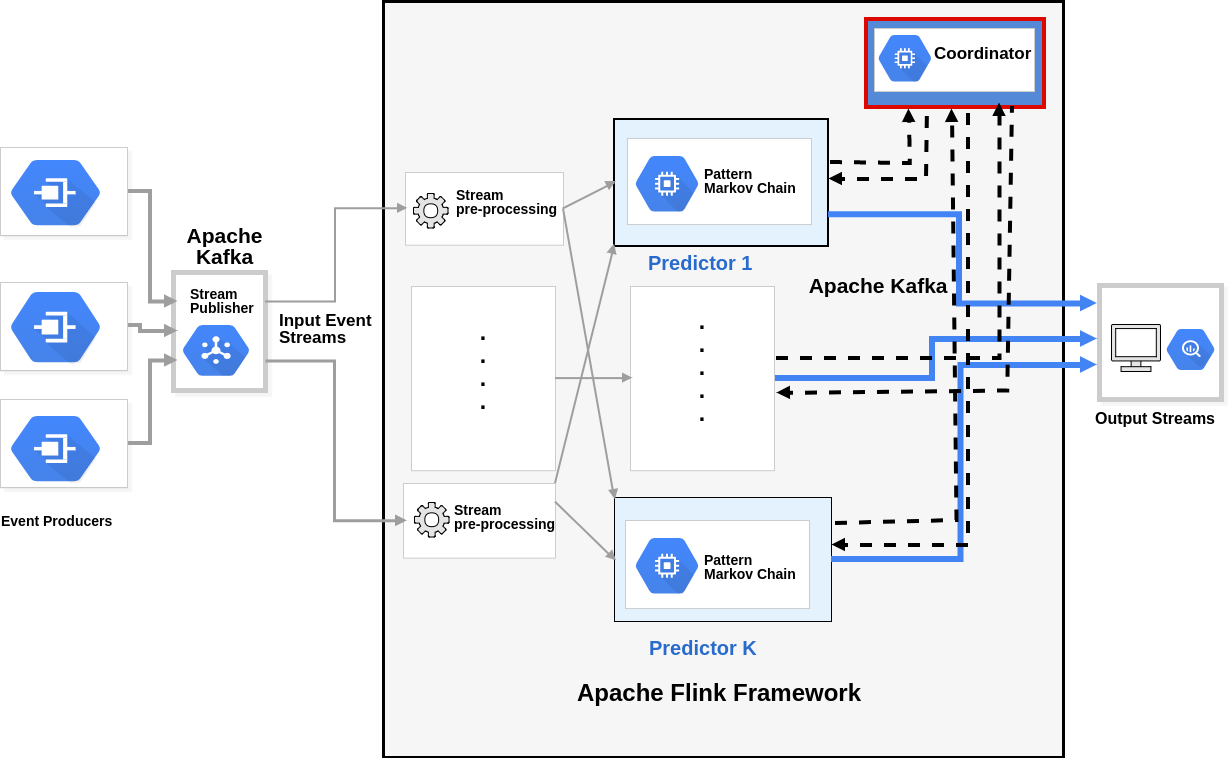
\includegraphics[width=\linewidth,left]{../chapters/figures/system.png}	\linebreak\\
	 .
		
%		emphasis on implementation // may add a slide // code link 
	\end{center}
}


\frame
{
	\frametitle{Scalable Pattern Prediction System \footnote{Source code: \url{https://goo.gl/BZ2Prk}.}}
	%\framesubtitle{Application Domain: Maritime Surveillance}
	\begin{itemize}
		
		\item<only@1> A scalable and distributed system that provides online pattern prediction over multiple real-time streams of events.
		\item<only@1> The proposed system is based on a novel method that combines  online probabilistic prediction models based on pattern Markov chain technique \cite{alevizos2017event} with a distributed online learning protocol \cite{kamp2014communication} to learn a global prediction model in a communication-efficient way.
		
	%	\item<only@1> The system maintains a Pattern Markov Chain prediction model for each event stream. 		
		\item<only@1> For large-scale processing support, the system is implemented on top of Apache Flink~\cite{carbone2015apache} along with Apache Kafka~\cite{Kafka}.
		
		%Apache Kafka is a scalable, fault-tolerant, and distributed streaming framework/messaging system \cite{Kafka}
		%on top of Apache Flink, a popular engine for distributed and large-scale stream processing. 
		\item<only@1> Developed in the context of the datAcron project \footnote{http://www.datacron-project.eu/}.
	\end{itemize}
}